\documentclass{article}
\usepackage[utf8]{inputenc}

\usepackage{amsmath}
\usepackage{amssymb}
\usepackage[top=1in, bottom=1in, left=1in, right=1in]{geometry}
\setlength{\parindent}{0em}
\setlength{\parskip}{1em}

\usepackage{multicol}

\usepackage{tikz}
\usepackage{pgfplots}
\usepackage{caption}

\usepackage{float}
\usepackage{caption}

\newcommand{\figref}[1]{Figure \ref{#1}}


\title{EECS 560 - Lab \#9}
\author{Theodore Lindsey}

\date{October 17, 2015}

\begin{document}

\maketitle


\section{Overall Organization of Experiment}
For this lab, we attempt to evaluate whether a skew heap or a leftist heap performs more quickly 
provided the same records are inserted into both tables.  We also attempt to evaluate which type of 
heap performs random inserts and deletemins more efficiently.





\section{Data Generation}
In this experiment, it is necessary that we insert the same values into both the leftist heap and 
the skew heap in order to achieve an apple-to-apples comparison.  To this end, we will use identical 
seeds for our pseudo random number generator in order to ensure that the same sequence of ``random'' 
numbers are inserted into both heaps.

In order to reduce variation in the results, multiple trials are run for each quantity of records.  
Each trial uses a different seed in order to reduce the impact of troublesome values to be inserted 
that might occur from a particular seed.  Each of the seeds used is the same for corresponding 
trials in each record quantity group.

Additionally, following a uniform distribution, the testing function randomly either inserts random 
records into the heap or deletes the minimum value from the heap.  The insertions are interspersed 
with the deletemin operations in order to maintain, roughly, the size of the heap.

Timing is measured by the provided timer class.  Times for individual runs are are recorded in the 
log file (`log.csv').  Averages for a specific quantities of records and merge method are calculated 
after running each experiment.  The averages are then displayed to console. Averages aren't recorded 
in the log file in order to make it easier and cleaner to import into a database or spreadsheet.






\section{Summary of Results (CPU Timing)}
In all trials, the skew heap had better performance than the corresponding leftist heap (as seen in 
each of the figures).






\section{Observation and Conclusion}
As noted in the previous section, the skew heap had better performance in both the build and insert/
deletemin trials. This is probably because it takes more work to compute and then compare rank in 
order to decide if a swap is needed than it is to just swap every time.  This is also consistent 
with what we learned from lecture.






\section{Data}

\begin{minipage}{0.49\textwidth}
    \begin{center}
        \begin{tabular}{|cccc|}\hline
        Seed & $n$ & Leftist & Skew    \\
        0 &  50000 & 0.01652 & 0.01125 \\
        1 &  50000 & 0.01521 & 0.01068 \\
        2 &  50000 & 0.01477 & 0.01049 \\
        3 &  50000 & 0.01558 & 0.01074 \\
        4 &  50000 & 0.01452 & 0.01036 \\
        5 &  50000 & 0.01578 & 0.01056 \\
        \multicolumn{2}{|c}{\textbf{avg}} & \textbf{0.01540} & \textbf{0.01068} \\ \hline
        0 & 100000 & 0.03346 & 0.02436 \\
        1 & 100000 & 0.03139 & 0.02399 \\
        2 & 100000 & 0.03229 & 0.02510 \\
        3 & 100000 & 0.03160 & 0.02495 \\
        4 & 100000 & 0.03148 & 0.02391 \\
        5 & 100000 & 0.03156 & 0.02417 \\
        \multicolumn{2}{|c}{\textbf{avg}} & \textbf{0.03196} & \textbf{0.02441} \\ \hline
        0 & 200000 & 0.06861 & 0.05192 \\
        1 & 200000 & 0.06434 & 0.05501 \\
        2 & 200000 & 0.06724 & 0.05810 \\
        3 & 200000 & 0.06598 & 0.05643 \\
        4 & 200000 & 0.06642 & 0.05654 \\
        5 & 200000 & 0.06807 & 0.05904 \\
        \multicolumn{2}{|c}{\textbf{avg}} & \textbf{0.06678} & \textbf{0.05617} \\ \hline
        0 & 400000 & 0.15191 & 0.11320 \\
        1 & 400000 & 0.12701 & 0.11636 \\
        2 & 400000 & 0.13138 & 0.11915 \\
        3 & 400000 & 0.13366 & 0.11474 \\
        4 & 400000 & 0.13650 & 0.10079 \\
        5 & 400000 & 0.12776 & 0.11127 \\
        \multicolumn{2}{|c}{\textbf{avg}} & \textbf{0.13470} & \textbf{0.11258} \\ \hline
        \end{tabular}
        \captionof{figure}{Build times with 5 \\ seed trials per value of $n$.}
        \label{tab:build}
    \end{center}
\end{minipage}
\begin{minipage}{0.49\textwidth}
    \begin{center}
        \begin{tabular}{|cccc|}\hline
        Seed & $n$ & Leftist & Skew    \\
        0 & 50000 & 0.00369 & 0.00197 \\
        1 & 50000 & 0.00374 & 0.00197 \\
        2 & 50000 & 0.00378 & 0.00197 \\
        3 & 50000 & 0.00375 & 0.00196 \\
        4 & 50000 & 0.00376 & 0.00195 \\
        5 & 50000 & 0.00377 & 0.00195 \\
        \multicolumn{2}{|c}{\textbf{avg}} & \textbf{0.00375} & \textbf{0.00196} \\ \hline
        0 & 100000 & 0.00819 & 0.00450 \\
        1 & 100000 & 0.00828 & 0.00451 \\
        2 & 100000 & 0.00833 & 0.00453 \\
        3 & 100000 & 0.00835 & 0.00450 \\
        4 & 100000 & 0.00840 & 0.00451 \\
        5 & 100000 & 0.00838 & 0.00452 \\
        \multicolumn{2}{|c}{\textbf{avg}} & \textbf{0.00832} & \textbf{0.00451} \\ \hline
        0 & 200000 & 0.01808 & 0.01014 \\
        1 & 200000 & 0.01826 & 0.01005 \\
        2 & 200000 & 0.01836 & 0.01006 \\
        3 & 200000 & 0.01978 & 0.01007 \\
        4 & 200000 & 0.01853 & 0.01006 \\
        5 & 200000 & 0.01851 & 0.01003 \\
        \multicolumn{2}{|c}{\textbf{avg}} & \textbf{0.01859} & \textbf{0.01007} \\ \hline
        0 & 400000 & 0.04229 & 0.02038 \\
        1 & 400000 & 0.03797 & 0.02006 \\
        2 & 400000 & 0.03838 & 0.02002 \\
        3 & 400000 & 0.03862 & 0.02001 \\
        4 & 400000 & 0.06750 & 0.02015 \\
        5 & 400000 & 0.03837 & 0.02000 \\
        \multicolumn{2}{|c}{\textbf{avg}} & \textbf{0.04385} & \textbf{0.02010} \\ \hline
        \end{tabular}
        \captionof{figure}{Insertion and deletemin times \\ with 5 seed trials per value of $n$.}
        \label{tab:ops}
    \end{center}
\end{minipage}




\section{Visualisation of Data}

\figref{fig:build} shows the average completion times for building the heaps for each seed for a 
given number of records.  \figref{fig:ops} shows the average completion times for each seed for 
performing insertions and deletemin operations for a given number of records.  As seen in the 
figures below, the results of this experiment are consistent with what we expected from the 
discussion in lecture.

\begin{figure}[H]
\centering

\begin{minipage}{0.45\textwidth}
    \centering
    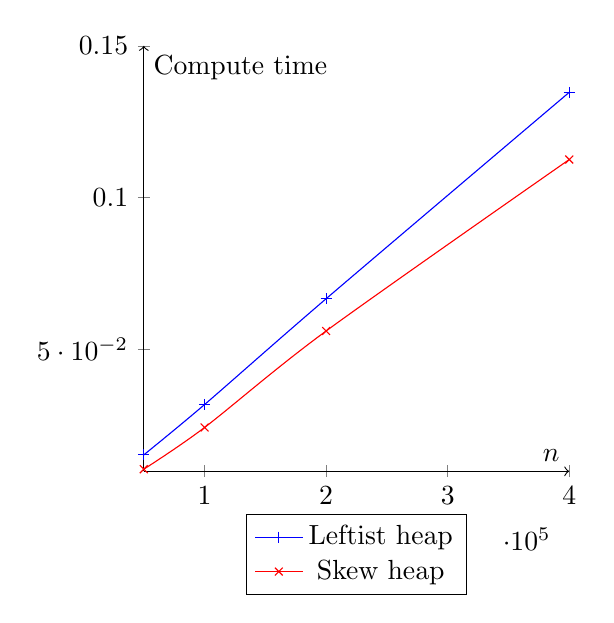
\begin{tikzpicture}
        \begin{axis}[
            width=2.75in,
            height=2.75in,
            xmin=50000,
            xmax=400000,
            ymin=0.01,
            ymax=0.15,
            axis lines=middle,
            axis line style={->},
            xlabel=$n$,
            ylabel=Compute time,
            legend style={at={(0.5,-0.1)},anchor=north}]
            
        \addplot[smooth,blue,mark=+] plot coordinates {
            (  50000 , 0.01540 )
            ( 100000 , 0.03196 )
            ( 200000 , 0.06678 )
            ( 400000 , 0.13470 )
        };
        \addlegendentry{Leftist heap}
    
        \addplot[smooth,color=red,mark=x] plot coordinates {
            (  50000 , 0.01068 )
            ( 100000 , 0.02441 )
            ( 200000 , 0.05617 )
            ( 400000 , 0.11258 )
        };
        \addlegendentry{Skew heap}
        \end{axis}
    \end{tikzpicture}
    \captionof{figure}{Building times.}
    \label{fig:build}
\end{minipage}
\begin{minipage}{0.45\textwidth}
    \centering
    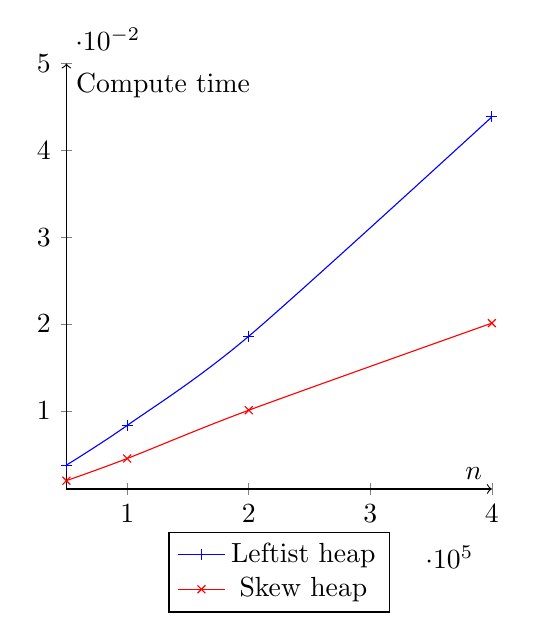
\begin{tikzpicture}
        \begin{axis}[
            width=2.75in,
            height=2.75in,
            xmin=50000,
            xmax=400000,
            ymin=0.001,
            ymax=0.05,
            axis lines=middle,
            axis line style={->},
            xlabel=$n$,
            ylabel=Compute time,
            legend style={at={(0.5,-0.1)},anchor=north}]
            
        \addplot[smooth,blue,mark=+] plot coordinates {
            ( 50000 , 0.00375 )
            ( 100000 , 0.00832 )
            ( 200000 , 0.01859 )
            ( 400000 , 0.04385 )
        };
        \addlegendentry{Leftist heap}
    
        \addplot[smooth,color=red,mark=x] plot coordinates {
            ( 50000 , 0.00196 )
            ( 100000 , 0.00451 )
            ( 200000 , 0.01007 )
            ( 400000 , 0.02010 )
        };
        \addlegendentry{Skew heap}
        \end{axis}
    \end{tikzpicture}
    \captionof{figure}{Insert / deletemin times.}
    \label{fig:ops}
\end{minipage}
\end{figure}
    



\end{document}